\documentclass[conference]{IEEEtran}
\IEEEoverridecommandlockouts
% The preceding line is only needed to identify funding in the first footnote. If that is unneeded, please comment it out.

% add this package to use [H]
\usepackage{float}

\usepackage{cite}
\usepackage{amsmath,amssymb,amsfonts}
\usepackage{algorithmic}
\usepackage[ruled]{algorithm2e}
\usepackage{graphicx}
\usepackage{subcaption}
\usepackage{textcomp}
\graphicspath{{images/}}
\def\BibTeX{{\rm B\kern-.05em{\sc i\kern-.025em b}\kern-.08em
    T\kern-.1667em\lower.7ex\hbox{E}\kern-.125emX}}
\begin{document}

\title{CS 289A Final Project\\
Human Driving Behavior Recognition and Prediction for a Ramp Merging Scenario
}
\author{
\IEEEauthorblockN{Hengbo Ma}
\IEEEauthorblockA{\textit{SID : 3033121067} \\
hengbo\_ma@berkeley.edu}
\and
\IEEEauthorblockN{Jessica Leu}
\IEEEauthorblockA{\textit{SID : 3033088125} \\
jess.leu24@berkeley.edu}
\and
\IEEEauthorblockN{Franklin Zhao}
\IEEEauthorblockA{\textit{SID : 3033030808} \\
qingan\_zhao@berkeley.edu}
\and
\IEEEauthorblockN{Yujun Zou}
\IEEEauthorblockA{\textit{SID : 27004846} 
\\
yujun\_zou@berkeley.edu}
}

\maketitle
\begin{abstract}
Prediction and recognition in complex situation have significant influence on the overall performance of autonomous driving systems. Many works focusing on single driver's behavior have been done. However, modeling multi-driver interaction, which is a more general case, is harder. In our project, we first divide human driving behavior into a hierarchical model which contains decision-making phase and maneuver phase. Next, we use classifiers to find the drivers' high-level intention, i.e., decision making, and then, we use Gaussian Mixture Models to capture different human driving behavior given their high level decisions. Last, base on the assumption that decisions in training data are unknown to us, we use a variational autoencoder to learn the representation of different driver behavior models in latent space and make prediction accordingly. A simulation data set from ramp-merging scenario is used to verify each models.    
\end{abstract}


\section{Introduction}
Prediction for human driving behavior is a significant part of autonomous driving system. The prediction can be seen as a prior knowledge for risk assessment before decision making and motion planning, etc. The importance of prediction further increases when the environment is more dynamic, complicated, and includes interactions. Many proposed methods mainly focus on ego car's recognition and prediction of human drivers' behavior \cite{ref:1,ref:2,ref:3,ref:4}. Recently, some work have been done to model the joint behavior of multiple drivers. In \cite{ref:5}, a review on motion prediction and risk assessment are provided. The authors proposed that the models that involves more interaction factors are important for danger detection and decision making system. Two kinds of typical interaction scenarios are shown in Figure~\ref{fig:interScen}.
\begin{figure}[h]
	\centering
	\begin{subfigure}[b]{0.2\textwidth}
		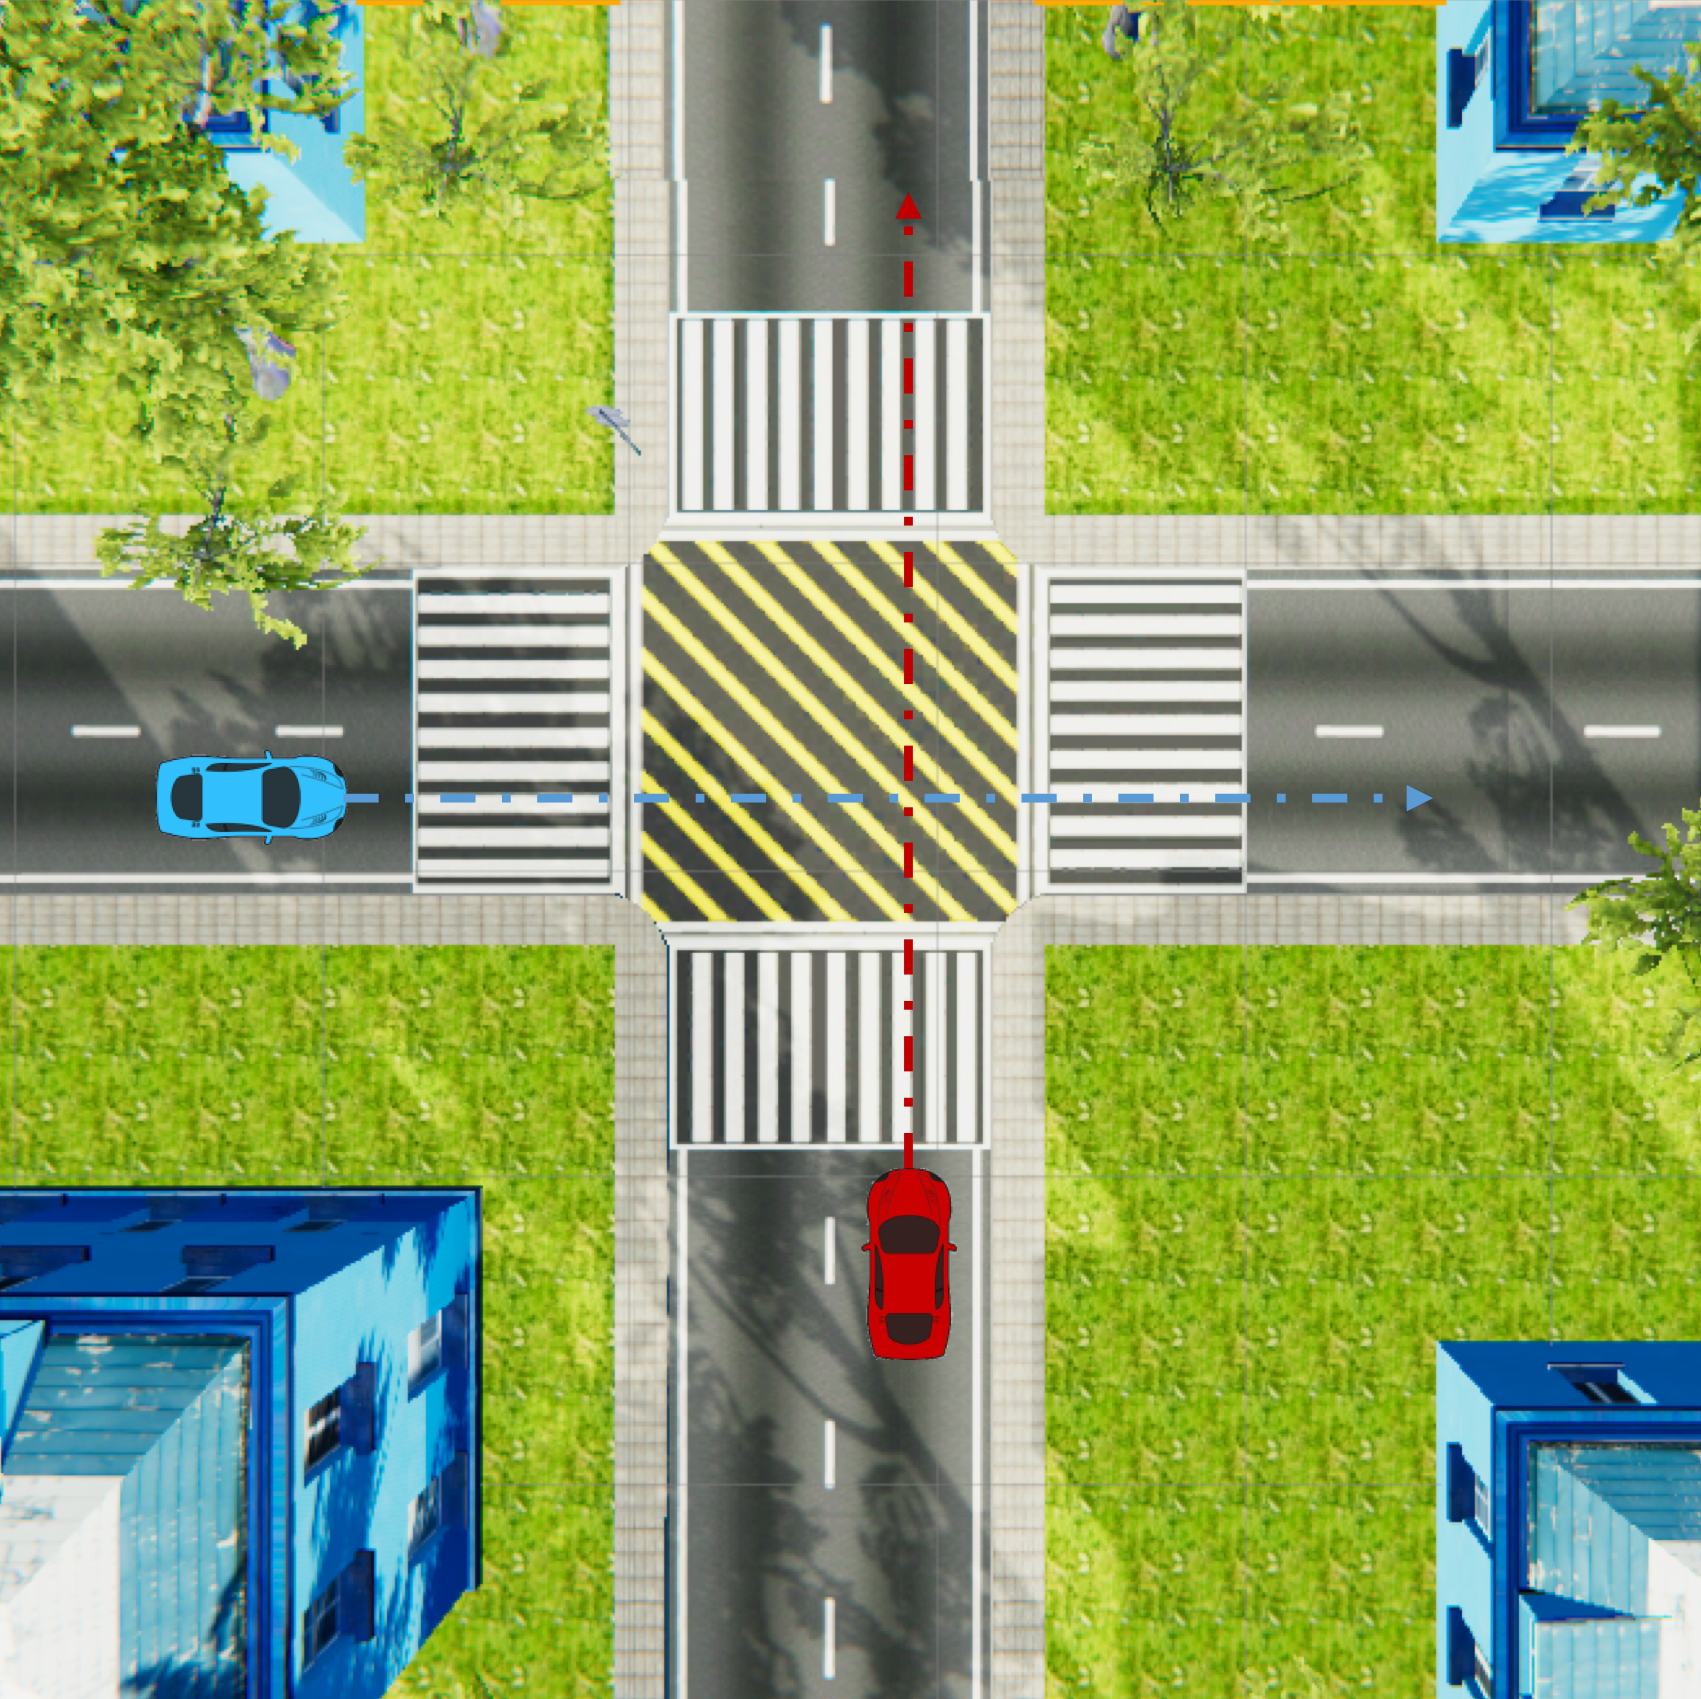
\includegraphics[width=1\textwidth]{scene1.png} 		
	\end{subfigure}
	\
	\begin{subfigure}[b]{0.2\textwidth}
		\includegraphics[width=1\textwidth]{scene2.png}
	\end{subfigure}
	\caption{Two kinds of typical interaction scenarios}
	\label{fig:interScen}
\end{figure}

In one recent research \cite{ref:6}, the author describes vehicle motions as seven high-level motion patterns, and regard the intention recognition as a classification problem. However, prediction for future motion is not included. In \cite{ref:7}, the authors introduced a Hidden Markov Model (HMM) and Gaussian process model to describe one driver behavior. 

Aside from using the probabilistic graph models, variational autoencoder is a method that has been used to imitate human behavior. In \cite{ref:8}, a variational inference based method was proposed to learn the latent-space representation of the human driving behavior pattern, and use it to imitate human behavior. However, no prediction phase was mentioned in the paper. In \cite{ref:9}, a stochastic variational method was proposed to predict a short video, which combines the power of convolutional neural network, recurrent neural network, and probabilistic model. They transfer the current image to next the image directly.
Besides, other works \cite{ref:10,ref:11,ref:12} also used variational method to describe the time sequence data.

In our work, in order to prediction human driving behavior and the future trajectory of the cars in the multi-agents system, we use a two-stage framework, containing decision making stage and maneuver stage, to predict the transition probability of the next state given the current state and the decision making output. In this framework, we tried several methods to model drives' behavior. We also design a variational autoencoder which is similar to the work in \cite{ref:8} but has the ability to predict future trajectory of the cars.

 
The reminder of this paper will be organized as follow: we formulate the problem in Section II. In Section III we introduce some methods for two the stages: decision making and maneuver learning, and also, for variational autoencoder. We then introduce the data which we used in Section IV. In Section V we talk about the experiment results and some discussion. Finally conclude our work and results. 

\section{Problem Formulation}
In order to learn human driving behavior, we use a dynamic bayesian network to represent the multi agents dynamic system. We concatenate the ego car's state and the environment cars' states to be the state in our system. The current state $S_t$ of the system is not only related to the previous state $S_{t-1}$, but also related to the input variable, $U_t$. We assume that the input variable is dependent on human drivers' observations of the current state $S_t$ and a latent variable $z$. Intuitively, the latent variable may represent the drivers' driving characters, such as being aggressive, conservative, or neutral. we divided the human driving model into two parts, decision making phase and maneuver learning phase. Decision making phase reflects whether a driver would like to yield to the main lane driver or not. We denotes this binary variable as $z_t$. For different decision, we use Markov chain to describe the human drivers' behaviors. We describe the multi-drivers scenario as a dynamic system. We assume that the relationship between the input variable and the state is linear:
\begin{equation}
s_{t} = As_{t-1} + Bs_{t-1}
\end{equation}

The dynamic bayesian network is shown in Figure~\ref{fig:dbn}:

\begin{figure}[H]
	\centering
	\includegraphics[width = 0.25\textwidth]{dbn.png}
	\caption{Dynamic bayesian network}
	\label{fig:dbn}
\end{figure}


where the state $S_{t}$ stacks each driver's state $s_{t}^{i}, i = 1, 2, \dots, n$:

\begin{align}
S_{t}=
\begin{bmatrix}
s_{t}^{1}, s_{t}^{2}, \dots, s_{t}^{n}
\end{bmatrix}
\end{align}

and the input $U_{t}$ stacks each driver's action $u_{t}^{i}, i = 1, 2, \dots, n$. $W_t$ and $V_t$ are the unknown noise signals .




\section{Methology}
\subsection{Decision Making Procedure}
\subsubsection{QDA, lDA and SVM}
This driving motion prediction problem is a two-class supervised classification problem, thus, we ran several baseline models to set baseline comparisons to our proposed HMM model. Models such as Quadratic Discriminant Analysis (QDA), Linear Discriminant Analysis (LDA), logistic regression (LR), and random forest (RF) are implemented with Scikit-learn package \cite{QIS1} and with default parameters in this project. Among all the baseline models, LDA achieved the best test accuracy at 91\%. Additionally, inspired by a recent paper in Neural Information Processing Systems (NIPS), we also implemented the LightGBM. Details will be discussed in the following part.

a. QDA and LDA

Quadratic Discriminant Analysis (QDA) is a specific generative method in which the class conditional probability distributions are independent Gaussians: $\mathcal{N} (\mu_k, \Sigma_k)$. Both parameters are estimated from the training set.
\begin{equation}
\hat{\mu}_k=\frac{1}{n_k}\sum_{t_i=k}x_i
\end{equation}
\begin{equation}
\hat{\Sigma}_k=\frac{1}{n_k}\sum_{t_i=k}(x_i-\hat{\mu}_k)(x_i-\hat{\mu}_k)^T
\end{equation}

LDA is a simplified version of QDA which assumes that all of the distributions share the same covariance matrix $\Sigma$. This is a simplification which, in the context of the Bias-Variance trade-off, increases the bias of our method but may help decrease the variance. Later we can see from the result that QDA over fits the training set, resulting a huge gap between the test set. 

b.	Logistic Regression 

Logistic Regression is a discriminative classification technique that has a direct probabilistic interpretation. In binary logistic regression, we would like our model to output the probability of a data point being in class 0 or 1. We started with raw data score $w^Tx$ and convert it to a probability between 0 and 1 by applying a sigmoid transformation $s(w^Tx)$, where $s(z) = 1/(1+e^{-z})$. Then, we classify $x$ as the class with maximum probability: 
\begin{equation}
\hat{y}=\max_kP(\hat{Y}=k|x,w)=\left\{
\begin{array}{cl}
1&\text{for }s(w^Tx)\geq 0.5\\
0&\text{otherwise}
\end{array}
\right.
\end{equation}

c. Random Forest

Random forests are a specific ensemble method where the individual models are decision trees trained in a randomized way so as to reduce correlation among them. In each decision tree, the loss function is called ``gini" impurity, which is defined as follow:
\begin{equation}
\begin{array}{rl}
G(Y)&=\sum_kP(Y=k)\sum_{j\neq k}P(Y=j)\\
&=\sum_kP(Y=k)(1-P(Y=k))\\
&=1-\sum_kP(Y=k)^2
\end{array}
\end{equation}

d. Light Gradient Boosting Machine (LGBM)

Boosting is another kind of ensemble method. The idea of boosting is to combine weak models to build a more robust one. In each iteration, miss-classified labels are assigned with higher weights so that the new model will have higher chance to classify it correctly. LGBM propose two novel techniques: Gradient-based One-Side Sampling (GOSS) and Exclusive Feature Bundling (EFB) to save the training efficiency \cite{QIS2}.

\subsubsection{Hidden Markov Model}
The Hidden Markov Model (HMM) is a statistical model originally proposed by Baum et. al. \cite{hmm1}, which is used for describing a Markov process with unobserved states \cite{hmm2}. The most crucial part when applying this model is to identify the hidden states from the observed states, so that the hidden states can be used for further analysis, e.g., pattern recognition. 

In normal Markov Models, all states are visible to the observer, therefore, the only parameter is the transition probability. However, in HMM, the states are not directly visible, while the variables (or let us say, outputs) that depend on those states are visible. Each of hidden state has a probability distribution over those outputs. Hence, the state can be analyzed and identified using the outputs which include some information of the hidden states.

Figure~\ref{fig:HMMmodel} illustrates the states change in HMM. Denote the state in time $t$ as $q(t)$ and the observation as $o(t)$. From the arrows we know that $q(t)$ is related to $q(t-1)$; $q(t-1)$ is related to $q(t-2)$, and so forth, while $o(t)$ is only related to the corresponding $q(t)$. It is obvious that in this architecture, $q(t)$ is the hidden state and $o(t)$ is the output. If there are $N$ possible values for $x(t)$, then $x(t+1)$ would have $N$ possible values as well ($N = 2$ in our case). Thus, there are $N^2$ possibilities from $t$ to $(t+1)$. If there are $M$ possible values for the observed $o(t)$, then the model complexity of $q(t)$ to $o(t)$ is $O(MN)$. If $o(t)$ is a $M$-dimensional vector, then the complexity would be $O(M^2N)$.
\begin{figure}[H]
	\centering
	\includegraphics{HMMmodel.pdf}
	\caption{Architecture of an instatiated HMM}
	\label{fig:HMMmodel}
\end{figure}

Given a HMM length $m$, denote the output as $O=\{o_1, o_2,\dots o_m\}$; hidden state as $Q=\{q_1, q_2,\dots q_m\}$. The probability model of an HMM can be described as:
\begin{equation}
P(o)=\sum_{Q}P(o|q)P(q)
\end{equation}

First denote the HMM parameters as $\lambda$ that contains 5 elements $(S,V,A,B,\pi)$, where $S$ represents the state set and $q(t)\in S$ ($S=\{0,1\}$ in our case); $V$ represents the output set and $o(t)\in V\ (t\in[1,T])$; $B=b_j(k)$ represents the probability distribution of the output ($b_j(k)=P(v_k|j),k\in[1,M],j\in[1,N]$); $\pi$ represents the initial probability distribution.

Generally, there are 3 basic problems for HMM\cite{hmm4}: Given parameters $(S,V,A,B,\pi)$ and the output sequence $O=(o_1,o_2,\dots,o_T)$, compute the likelihood of the observations, namely $P(O|\lambda)$, which is an evaluation problem; Given parameters and the output sequence, find the most likely state sequence $Q=\{q_1, q_2,\dots q_m\}$ that produce the observations, which is a decoding problem; Given the output sequence, find the parameters $\lambda$ to maximize $P(O|\lambda)$, which is exactly the problem of our project -- learning problem. Expectation-maximization algorithm (EM) is applied to solve this kind of learning problem.

The expectation of our state variables is the probability that the state of a random variable $X$ is $i$ at time step $t$, namely $q(t)=i$. To calculate this probability, the forward variables $\alpha$, and backward variables $\beta$ are introduced.
\begin{equation}
\alpha_t(i)=P(o(1),o(2),\dots,o(t),q_t=i|\lambda)
\end{equation}
Namely, forward variables are the probability that the observations are $o(1),o(2),\dots,o(t)$ in state $i$ given $\lambda$ and time step $t$. Then the following equations can be derived:
\begin{equation}
\alpha_1(i)=\pi_ib_i(o_1),\ 1\leq i\leq N
\end{equation}
\begin{equation}
\alpha_{t+1}(j)=(\sum_{i=1}^N\alpha_t(i)a_{ij})b_jo_{t+1}, \ 1\leq t\leq T-1,\ 1\leq j\leq N
\end{equation}
\begin{equation}
P(O|\lambda)=\sum_{i=1}^N\alpha_T(i)
\end{equation}
Similarly, for backward variables we have:
\begin{equation}
\beta_t(i)=P(o(t+1),o(t+2),\dots,o(T),q_t=i|\lambda)
\end{equation}
\begin{equation}
\beta_T(i)=1,\ 1\leq i\leq N
\end{equation}
\begin{equation}
\beta_t(i)=\sum_{j=1}^Na_{ij}b_j(o_{t+1})\beta_{t+1}(j),\ 1\leq t\leq T-1,\ 1\leq i\leq N
\end{equation}
\begin{equation}
P(O|\lambda)=\sum_{i=1}^N\pi_ib_i(o_1)\beta_1(i)
\end{equation}
``E" step:

Denote the probability that the state is $i$ in time step $t$ and $j$ in time step $t+1$ given the parameters $\lambda$ and the observation sequence $O$ by $\xi_t(i,j)$. Then the following equation can be derived:
\begin{equation}
\begin{array}{rl}
\xi_t(i,j)=&P(q_t=i,q_{t+1}=j|O,\lambda)\\
=&\frac{P(q_t=i,q_{t+1}=j,O|\lambda)}{P(O|\lambda)}\\
=&\frac{\alpha_t(i)a_{ij}b_j(o_{t+1})\beta_{t+1}(j)}{P(O|\lambda)}\\
=&\frac{\alpha_t(i)a_{ij}b_j(o_{t+1})(j)}{\sum_{i=1}^N\sum_{j=1}^N\alpha_t(i)a_{ij}b_j(o_{t+1})\beta_{t+1}(j)}
\end{array}
\end{equation}
Denote the probability that the state is $i$ in time step $t$ given $\lambda$ and $O$ by $\gamma_T(i)$. Then the following equation can be derived:
\begin{equation}
\gamma_t(i)=\sum_{i=1}^N\xi_t(i,j),\ 1\leq t\leq T
\end{equation}
Plugging $t$ into these equations, the expectations of the times that state $i$ changed and the times that state $i$ turned to $j$ can be obtained.\\

\noindent ``M" step:

Denote the expectation of the frequency that $i$ is the initial state by $\bar{\pi}_i$, and we have:
\begin{equation}
\bar{\pi}_i=\gamma_1(i)
\end{equation}
Similarly, denote the expectation of the times that state $i$ turned to state $j$ devided by the expectation of the times that state $i$ changed by $\bar{a}_{ij}$, and we have:
\begin{equation}
\bar{a}_{ij}=\frac{\sum_{t=1}^{T-1}\xi_t(i,j)}{\sum_{t=1}^{T-1}\gamma_t(i)}
\end{equation}
where $\bar{b}_j(k)$ is the expectation of the times that output is $k$ in state $j$ divided by the expectation of the times that any other states turned into state $j$.
\begin{equation}
\bar{b}_j(k)=\frac{\sum_{t=1}^T\gamma_t(i)\delta(o_t,v_k)}{\sum_{t=1}^T\gamma_t(i)}
\end{equation}
\begin{equation}
\delta(o_t,v_k)=\left \{ 
\begin{array}{ll}
1&\text{for }o_t=v_k\\
0&\text{otherwise}
\end{array}
\right.
\end{equation}
Hence, parameters $\lambda=(A,B,\pi)$ will be updated, and the forward and backward variables can be computed again in each iteration. The loop will keep running until the parameters converge.\\


Next, we trained these two HMM model for different decision making strategies, we need to get the posterior likelihood of the current scenario. we can use softmax to get the probability: 

\begin{align}
p(x = i)  = \frac{e^{s_i}}{\sum_{i = 1}^{N}{e^{score_i}}}
\end{align}

However,because we optimize the log likelihood $p(x)$ in the training phase is, we will get different scale values for different HMM chain. Even within each HMM chain, we will get the relative probability. Therefore, when we combine two HMM together, normalization or a prior information is needed.

We assume that at the starting point of the road, after a short fixed length sliding window, the probability is 0.5. Then when we use HMMs to predict the decision, we will get two scores. We want to scale this two scores to 0.5, then we can get the final probability of the decision.


In this project, we implemented this algorithm and trained data using a Python package \textit{hmmlearn} \cite{hmm4}. 
\subsection{Maneuver Imitation Procedure}
\subsubsection{Gaussian Mixture Model}
Gaussian Mixture Model is very useful with data which has multi-model and complex structures. We assume that under each decision, we have a GMM to model the maneuver motion:

\begin{align}
p(U_{t}, S_{t} | Y = y) = \sum_{i = 1}^{N}{w_i\mathcal{N}(U_{t}, S_{t} | \mu_{i}, \sigma_{i}^{2}, Y)}
\end{align}

The prior probability $p(Y)$ will be obtained from the decision making phase.

Still, we use EM algorithm to estimate the parameters of the GMM model. After we get the joint distribution $p(U_{t}, S_{t} | Y)$, we are able to get the conditional probability $p(U_{t} | S_{t}, Y)$.

For each component of GMM , we have the mean and variance:
\begin{align}
\mu_{i}&=
\begin{bmatrix}
\mu_{i, U_{t}} &\mu_{i, S_{t}}\\
\end{bmatrix}\\
\Sigma_{i}&=
\begin{bmatrix}
\Sigma_{i, U_{t}} & \Sigma_{i, U_{t}, S_{t}}\\
\Sigma_{i, U_{t}, S_{t}} & \Sigma_{i, S_{t}}\\
\end{bmatrix}
\end{align}

Then we can get the conditional probability parameters:

\begin{align}
\mu_{i, U_{t} | S_{t}} &= \mu_{i, U_{t}} + \Sigma_{i, U_{t}}^{-1}(S_{t} - \mu_{i, S_{t}}\\
\Sigma_{i, U_{t} | S_{t}} &= \Sigma_{i, U_{t}} - \Sigma_{i, U_{t}}^{-1}\Sigma_{i, U_{t}, S_{t}}\\
w_{i | S_{t}} &= \frac{w_{i}p(S_{t} | \mu_i, \Sigma_i)}{\sum_{i=1}^{N}{p(S_{t} | \mu_i, \Sigma_i)}}
\end{align}

After we get all the parameters in these two parts, we use the decision making phase result, e.g. the probability of latent variable $y$ (the intention to yield or not yield) as the prior of the maneuver models. the final prediction will be drawn from the distribution:

\begin{align}
p(U_{t+1} | S_{t+1}) = \sum_{i = 0}^{1} p(U_{t+1} | S_{t}, Y = i )p(Y = i)
\end{align}

\subsection{Variational Autoencoders}

\begin{figure*}[t]
	\centering
	\includegraphics[width = 0.55\textwidth]{vae.png}
	\caption{Neural network architecture for training}
	\label{fig:nn}
\end{figure*}

The methods above is based on the assumption that labels of the training data are known. However, in the real world, it is hard to annotate them. Therefore, unsupervised learning method is needed. Nonetheless, we also want a probabilistic model rather than a deterministic model. Since the probability $p(s)$ is intractable, we cannot get the exact inference of the probability density function (pdf). There are several methods to approximate the pdf. Monte Carlo method gets the pdf by sampling the particles based on the hypothetical pdf model, and learning the parameters. Variational Inference is another technique for approximating the pdf \cite{ref:13,ref:14,ref:15}. Some related work on how to apply the variational Inference to imitating the driving behaviors has been done \cite{ref:8}. In the paper, authors learns the policy $\pi(u_{t} | s_{t})$. In our methods, we are going to learn the transition probability $p(s_{t+1} | s_{t})$. Consider the likelihood $p(s_{1:T}| s_{0})$, we have:

\begin{align}
p(s_{0:T}) &= p(s_{1:T} | s_{0})p(s_{0}) \\
p(s_{1:T} | s_{0}) &= \prod_{i = t}^{T}{p(s_{i} | s_{0:i-1}, z)}p(z | s_{i-1})\\
&= E_{z\sim p(z)}[ \prod_{i = 1}^{T}{p(s_{i} | s_{0:i-1}, z)} ]
\end{align}

In the above Equation, we assume that the latent variable $z$ is independent with a single state $s_{t}$. For convenience, we will denote $p = p(z)$ and $q = q(z | s_{0:T-1})$ for now. Considering the log-likelihood $L(s_{1:T}|s_{0}) = log(p(s_{1:T} | s_{0}))$:

\begin{align}
L(s_{0:T}) & = log(p(s_{1:T} | s_{0})) + log(p(s_{0}))
\end{align}

by using the Jensen Inequality:

\begin{equation}\label{eq:Jensen}
\begin{array}{rl}
&log(p(s_{1:T} | s_{0}))\\
= &logE_{z\sim p}[\prod_{i = t}^{T}{p(s_{i} | s_{0:i-1}, z)}]\\
\geq &\sum_{i = t}^{T}{ E_{z\sim p}[ log(p(s_{i} | s_{0:i-1}, z))] }\\
\geq &\sum_{i = t}^{T}{ E_{z\sim q}[ log(p(s_{i} | s_{0:i-1}, z)] + E_{z\sim q}[\frac{p(z)}{q(z | s_{0:T-1})})]} \\
\geq &\sum_{i = t}^{T}{ E_{z\sim q}[ log(p(s_{i} | s_{0:i-1}, z)]} - KL[q || p]
\end{array}
\end{equation}

Now if we optimize the lower bound of the loglikehood in the equation, we actually will get the lower bound of the loglikelihood.

From the dynamic bayesian network descirble in last section, we can assume that the $s_{t}$ doesn't depend on the state before t-1. Hence the right side of inequality (\ref{eq:Jensen}) will become the following:

\begin{equation}
\sum_{i = t}^{T}{ E_{z\sim q}[ log(p(s_{i} | s_{i-1}, z)]} - KL[q || p]
\end{equation}

\subsubsection{training Phase}

Recurrent Neural Network has great performance on capturing the inherent dynamics of a sequence of data. We use the Long Short Term Memory Recurrent Neural Network as the encoder to describe the probability $p(z | s_{0:t})$. When we get the parameters of the probability distribution, we use the reparameterization trick to sample the latent variable $z$. 

we assume that the probability $p \sim N(0, I)$. For the decoder part, we use the fully connected neural network to capture the probability density function $p(s_{t+1} | s_{t}, z)$, and we assume the pdf is a gaussian function. The output is the pdf's parameters. Similarly, we sample the $s_{t+1}$ based on the generated parameters. The whole process is illustrated in Figure~\ref{fig:nn}.

\subsubsection{Prediction Phase}

Once we trained the variational autoencoder, we will only use the encoder once. We sample the latent variable $z$ from the normal distribution. Given the current state $s_{t}$ we can get the sample $\hat{s_{t+1}}$. When we get the prediction $\hat{s_{t+1}}$, we will use this state as the next input of the decoder. This procedure will be repeated for $T$ times, where  $T$ is the prediction horizon. The algorithm is shown in Algorithm 1.



\begin{algorithm}
\KwResult{Write here the result }
initialize the sliding window length $l$\;
initialize the start point c of prediction sequence\;  
initialize traj[i][p] $\gets$ empty\;
\For{Particle p = 1 : M}{
  	$\hat{s}_{c-l:c} \gets {s}_{c-l:c}$\; 
\For{t = c: T}{
  	sample $z_i$ from pdf $p(z | \hat{s}_{c-l:c})$\;
  	calc pdf $p(\hat{u}_{t+1} | \hat{s}_{t}, z_i)$\;
  	get $p(\hat{s}_{t+1} | \hat{s}_{t}, z_i)$\;
   	sample $\hat{s}_{t+1}$\;
   	save $\hat{s}_{t+1}$ in traj[i][p]\;
 	$\hat{s}_{t} \gets \hat{s}_{t+1}$\;
 	$\hat{s}_{c-l:c} \gets [\hat{s}_{c-l+1:c}\ \hat{s}_{t+1}]$\; 	 	
   	}
 } 
\caption{Formulation of Algorithm 1}
\end{algorithm}

\section{Data Set and Data Processing}

There are many kinds of interaction between cars on road, such as signalized and unsignalized intersection, merging lane, roundabout, etc. Since signalized intersection has other information source such as traffic lights, it is out of scope for this paper and will not be discussed. However, there are only little amount of data for the remaining scenarios mentioned above. Even though NGSIM has the data which includes lane changing , car following, signalized intersection and merging lane, the resolution is too low and sometimes the ground truth is incorrect. In order to model the procedure of the car interaction with the real ground truth to evaluate it, we develop a simulator to simulate the scenario of the interaction. 

Since we don't have labeled data of the real world unsignalized intersection, we simulated the merging lane situation of which the real world data is also accessible. 

\subsection{Merging Scenario Simulation}
In the simulation settings, we assume that both main-lane car and merging car are free to run, which means that the preceding cars are far away enough so that we only need to consider the main-lane car and the merging car in this scenario. 

In simulation, both cars are driven by human drivers who will manipulated the car through Logitech G920 gaming wheel and pedals. We wrote the simulation in Unity3D, which has a powerful physics engine and rendering engine. The human drivers can observe the environment from the car's front window, left and right blind spot mirrors, and the rear-view mirror same as in the real world.

The two cars are initialized at the same time, and we assume that the two cars' initial speeds are around 30 mph, when the merging procedure is finished, the data is recorded. An example of the recorded data is illustrated in Figure~\ref{fig:mergeRec}.

\begin{figure*}[t]
	\centering
	\includegraphics[scale=0.4]{scene_real.png}
	\caption{Recorded merging procedure}
	\label{fig:mergeRec}
\end{figure*}

For each car, we recorded the car's position (including the longitudal and lateral coordinate), yaw angle, and the velocity (including the longitudal and lateral coordinate). we also calculated the relative displacement of two cars, such as the relatively position and relatively velocity. The features are set in the way illustrated in Figure~\ref{fig:mergeFeat} and Table~\ref{tb:mergeFeat}.

\begin{figure}[H]
	\centering
	\includegraphics[scale=0.1]{coordi.png}
	\caption{Merging feature visualization}
	\label{fig:mergeFeat}
\end{figure}

\begin{table}
\centering
\caption{Merging feature}\label{tb:mergeFeat}
\begin{tabular}{c | c}

\hline
features &  meaning\\
\hline
$x_{1}$ & car1's position along with the x axis\\
$y_{1}$ & car1's position along with the y axis\\
$v^x_{1}$ & car1's velocity along with the x axis\\
$v^y_{1}$ & car1's velocity along with the y axis\\
$x_{2}$ & car2's velocity along with the x axis\\
$y_{2}$ & car2's velocity along with the y axis\\
$v^x_{2}$ & car2's velocity along with the x axis\\
$v^y_{2}$ & car2's velocity along with the y axis\\
$v_r$ & relative velocity between car1 and car2\\
$x_r$ & relative position along x axis between car2 and car1\\
$y_r$ & relative position along y axis between car2 and car1\\
\hline
\end{tabular}
\end{table}

Figure~\ref{fig:phase} is the phase graph to reflect the two cars interaction. The x axis represents the merging lane car's position as time moves on. The y axis represents the main lane car's position as time moves on. we only show 4 different interaction procedure in this figure.
\begin{figure}[h]
	\centering
	\includegraphics[scale = 0.35]{phase.png}
	\caption{Phase graph for the interaction}
	\label{fig:phase}
\end{figure}


\section{Experiment Results}
\subsection{Decision Making Procedure}
\subsubsection{Basic Models}
The results of the basic models are shown in Table~\ref{tb:QISresult} and Figure~\ref{fig:QISresult}.
\begin{table}[H]
	\caption{Result of basic models}
	\centering
	\label{tb:QISresult}
\begin{tabular}{lrr}
\hline
\textbf{Models} &           \textbf{Testing accuracy} &          \textbf{Training accuracy}\\
\hline
QDA &   48.379125 &  56.913947 \\
LDA &   90.703591 &  91.958457 \\
Logistic Regression &   90.652711 &  91.008902 \\
Random Forest &  100.000000 &  90.089021 \\
LGBM &  100.000000 &  92.195846 \\
\hline
\end{tabular}
\end{table}
\begin{figure}[H]
	\centering
	\includegraphics[scale = 0.3]{QISresult.png}
	\caption{Prediction results in one trajectory (true label: 1)}
	\label{fig:QISresult}
\end{figure}
As Table~\ref{tb:QISresult} shows, LDA gives the best result in terms of both overall accuracy and timing while QDA over fits the data. This is because in our model, the two classes represent the behavior of two drivers which are similar Gaussian distributions. Also, in the test set, we collect data from the same driver as the training set which makes it more suitable for LDA to achieve good result. In the QDA it assumes two different covariance matrix which will result in overfitting. However, if we collect data from multiple drivers, we expect that the accuracy of LDA will drop and QDA will increase. The result of logistic regression is also great. A higher accuracy from LDA indicates that our data falls in the category of Gaussian distribution with same class mean and variance thus linearly separable. As a result, logistic regression would also provide a high accuracy as it is also a linear based model. The performance of random forest is not that good since all the features are continuous whereas RF meant to predict categorical features.  

Other than the overall predicting accuracy, we also want our model to predict the labels as soon as possible so that we could make early decisions. The graph above shows the predicting probability in one testing trajectory along the time steps. LDA clearly was the first model that forecasts the correct labelling ahead of other models. LGBM also has a higher rate of accuracy while its forecasting probability is not as satisfactory in the early stage. During early stage, when the two cars are far away, we expect the model to give probabilities around 0.5 since there is little chance to predict the label from that time. LGBM provides wrong label and with high confidence which is undesired. Other models such as LR, RF, and QDA, have even worse performances than LGBM as the table and graph show. 

\subsubsection{HMM}

In this part, the hmm result has been shown in Figure~\ref{fig:hmmResult}. In this figure, we test a sample cases, which the true label is 1, we use a sliding window which has length 20 time steps to predict the probability of whether the merging lane car will yield to the main lane car.

We see that because we force the initial probability to be 0.5, which is useful for unify the two different HMM model, so that they can be adjusted immediately after new observation has been made. It is reasonable that in the last part of the road, the car will have high probability to a certain decision, because the merging stage is already finished, we know that the merging lane car yield to the main lane car.

\begin{figure}[H]
	\centering
	\includegraphics[scale = 0.6]{hmm_res.png}
	\caption{Result of HMM}
	\label{fig:hmmResult}
\end{figure}

From Figure~\ref{fig:hmmResult} and Figure~\ref{fig:QISresult}, we can conclude that the HMM has a slightly better result.
\subsection{Maneuver Learning Procedure}
In the maneuver learning procedure, we use two Gaussian Mixture Model to fit the joint probability described above. Here we use a 30 Gaussian kernels and train it for 1000 times. Then we use several test sample to validate the performance. Figure~\ref{fig:gmmResult} shows the 2 second long prediction:

\begin{figure}[h]
	\centering
	\includegraphics[scale = 0.2]{gmm_2s.png}
	\caption{Result of GMM}
	\label{fig:gmmResult}
\end{figure}

From the predict result, we found that the ground truth lies in the samples trajectories, and the prediction is basically correct. so we can combine it and with the HMM result from above to make a final prediction. \subsection{Varion iational Autoencoder}
We trained a recurrent variaitonal autoencoder defined above. For the encoder part, we use a 30 LSTM cell recurrent neural network, and for the decoder, we only use a two hidden layers fully connected neural network which each layer has 30 units. We separated the original data set into training data set and testing data set. Because we would like to let the encoder's input has fixed length, we divided the data set every fixed time steps. We use mini-batch stochastic gradient descent method, and each batch has 1000 samples. After 5000 iteration, the loss converged.
\begin{figure}[h]
	\centering
\begin{subfigure}[h]{\textwidth}
	\includegraphics[scale = 0.17]{vae_k_1_2s.png}
\end{subfigure}
\begin{subfigure}[h]{\textwidth}
	\includegraphics[scale = 0.17]{vae_k_1_4s.png}
\end{subfigure}
    \caption{HMM prediction}
	\label{fig:hmmPred}
\end{figure}

We use a testing trajectory to show the result of prediction in Figure~\ref{fig:hmmPred}. In this figure, we will see that the error is not so big, but the variance is too small. It seems that variational autoencoder will underestimate the variance.

Next we want to check the latent space to show how good the encoder is. Figure~\ref{fig:vae1} is the picture of the VAE with $\lambda = 1$, Figure~\ref{fig:vae0.02} is the picture of the VAE with $\lambda = 0.02$. From the results, we find that when using the original VAE, each latent variable behaves like a normal distribution, and they are entangled together. This means that the latent variable is uninformative. This kind of results has been discussed in several materials, \cite{ref:16,ref:17,ref:18,ref:19}, which says that the KL divergence is too restrictive, so the optimization will let the posterior likelihood $q(z | x)$ to be just $p(z)$, which is a normal distribution and not so useful for the decoder. Therefore, the decoder will not rely on the latent variable, and only rely on the current input $s_{t}$, which will ignore the encoder's efforts. 

When we tune the hyperparameter $\lambda$ in the loss function, as been done in the paper \cite{ref:8}, we do observe a relatively good latent space representation. From the figure, we can find that the two different cases are separated.

\begin{figure}[h]
	\centering
	\includegraphics[scale = 0.17]{vae_z_2.png}
	\caption{VAE with $\lambda=1$}
	\label{fig:vae1}
\end{figure}

\begin{figure}[h]
	\centering
	\includegraphics[scale = 0.3]{vae_z_1.png}
	\caption{VAE with $\lambda=0.02$}
	\label{fig:vae0.02}
\end{figure}


\section{Conclusion}
 In this report, we researched on how to predict and recognize human behavior by using different model. The first model we used is a two stage framework. We first predicted the human driver's intention by using several models like LDA, QDA, HMM, etc. Then we used the GMM model to describe the driver's maneuvers. We found that when using HMM model, the probability we got was much more reasonable then other models. For the maneuver learning, GMM captured the mean and variance well, but the difference between the different intention were small, which was not expected. This was because the EM algorithm captured the global feature but lost the details. Secondly, we used a variational autoencoder to desrible the whole procedure. We proposed a variational autoencoder combined with recurrent neural network to predict the furture motion. The result was decent in a relatively short time period. However, the variational autoencoder did't capture the variance of data very well, at the same time, the weight of KL divergence item in the loss function influenced the latent space representation learning performance. After we changed the weight of KL,  some improvement did show up. Finally, we implement several models to finish the task. In the future we will continue research on related materials.
%\section{Acknowledgement}

\bibliographystyle{IEEEtran}
\bibliography{reference}

\end{document}
